\documentclass[12pt,a4paper]{article}

% ─── Page Layout ───────────────────────────────────────────────────────────────
\usepackage[a4paper, margin=0.8in, headheight=14pt]{geometry}

% ─── Fonts (XeLaTeX) ───────────────────────────────────────────────────────────
\usepackage{fontspec}
\usepackage{unicode-math}
\setmainfont{TeX Gyre Pagella}
\setmonofont[Scale=0.88]{TeX Gyre Cursor}
\setmathfont{Latin Modern Math}

% ─── Packages ──────────────────────────────────────────────────────────────────
\usepackage{xcolor}
\usepackage{colortbl}
\usepackage{titlesec}
\usepackage{enumitem}
\usepackage{tabularx}
\usepackage{booktabs}
\usepackage{array}
\usepackage{amsmath}
\usepackage{tikz}
\usetikzlibrary{shapes.geometric, arrows.meta, positioning, calc, fit, decorations.pathreplacing}
\usepackage{tcolorbox}
\tcbuselibrary{skins, breakable}
\usepackage{hyperref}
\usepackage{fancyhdr}
\usepackage{graphicx}
\usepackage{microtype}
\hyphenpenalty=10000
\exhyphenpenalty=10000
\sloppy
\usepackage{caption}
\usepackage{setspace}
\usepackage{multirow}
\usepackage{tocloft}

% ─── Q&A helper ────────────────────────────────────────────────────────────────
\newcommand{\Q}[1]{\textbf{#1}\par\noindent\ignorespaces}

% ─── Colour Palette ────────────────────────────────────────────────────────────
\definecolor{myred}{RGB}{196,30,58}
\definecolor{mydark}{RGB}{30,30,50}
\definecolor{mygreen}{RGB}{14,120,80}
\definecolor{myteal}{RGB}{0,130,140}
\definecolor{myamber}{RGB}{180,100,0}
\definecolor{mypurple}{RGB}{100,30,160}
\definecolor{mygray}{RGB}{246,247,249}
\definecolor{mgframe}{RGB}{180,185,200}
\definecolor{watermark}{RGB}{145,150,170}
\definecolor{hdrred}{RGB}{250,232,235}
\definecolor{hdrgreen}{RGB}{220,244,233}
\definecolor{hdrteal}{RGB}{220,242,244}
\definecolor{hdramber}{RGB}{253,242,215}
\definecolor{hdrpurple}{RGB}{238,228,255}
\definecolor{hdrgray}{RGB}{238,240,245}
\definecolor{rowalt}{RGB}{250,251,253}

% ─── Section Formatting ────────────────────────────────────────────────────────
\titleformat{\section}
  {\large\bfseries\color{myred}}{\thesection.}{0.5em}{}
  [\vspace{1pt}{\color{myred}\rule{\linewidth}{0.8pt}}]
\titleformat{\subsection}
  {\normalsize\bfseries\color{myteal}}{\thesubsection}{0.5em}{}
\titlespacing*{\section}{0pt}{18pt}{7pt}
\titlespacing*{\subsection}{0pt}{11pt}{4pt}

% ─── Paragraph ─────────────────────────────────────────────────────────────────
\setlength{\parindent}{0pt}
\setlength{\parskip}{4pt}

% ─── TOC Styling ───────────────────────────────────────────────────────────────
\renewcommand{\cfttoctitlefont}{\large\bfseries\color{myred}}
\renewcommand{\cftaftertoctitle}{\par\noindent{\color{myred}\rule{\linewidth}{0.8pt}}}
\setlength{\cftbeforetoctitleskip}{0pt}
\setlength{\cftaftertoctitleskip}{6pt}
\renewcommand{\cftsecfont}{\normalsize\bfseries\color{mydark}}
\renewcommand{\cftsecpagefont}{\normalsize\bfseries\color{mydark}}
\renewcommand{\cftsecleader}{\cftdotfill{\cftdotsep}}
\setlength{\cftbeforesecskip}{7pt}
\renewcommand{\cftsubsecfont}{\small\color{mydark}}
\renewcommand{\cftsubsecpagefont}{\small\color{mydark}}
\setlength{\cftbeforesubsecskip}{3pt}
\setlength{\cftsubsecindent}{1.4em}

% ─── Table helpers ─────────────────────────────────────────────────────────────
\renewcommand{\arraystretch}{1.45}
\setlength{\tabcolsep}{6pt}
\arrayrulecolor{mydark}
\newcolumntype{B}[1]{>{\small\bfseries\raggedright\arraybackslash}m{#1}}
\newcolumntype{Y}{>{\small\raggedright\arraybackslash}X}
\renewcommand{\tabularxcolumn}[1]{m{#1}}

% ─── Header / Footer ───────────────────────────────────────────────────────────
\pagestyle{fancy}
\fancyhf{}
\fancyhead[L]{\small\color{myred}\textbf{PE-EC702B}\;\color{mydark}--- Digital Image and Video Processing}
\fancyhead[R]{\small\color{myteal}\textbf{Module 8 Notes}}
\fancyfoot[C]{\small\color{mydark}\thepage}
\fancyfoot[R]{\small\color{watermark}\textit{\copyright\ Biraj}}
\renewcommand{\headrulewidth}{0.5pt}
\renewcommand{\footrulewidth}{0.3pt}

% ─── Hyperref ──────────────────────────────────────────────────────────────────
\hypersetup{
  colorlinks=true, linkcolor=myteal, urlcolor=myteal,
  pdfauthor={Biraj Sarkar},
  pdftitle={PE-EC702B --- Module 8 Notes}
}

% ─── tcolorbox styles ──────────────────────────────────────────────────────────
\tcbset{
  tikzbox/.style={
    colback=mygray, colframe=mgframe, boxrule=0.6pt, arc=4pt,
    left=8pt, right=8pt, top=6pt, bottom=6pt,
    colbacktitle=mgframe, coltitle=mydark,
    fonttitle=\small\bfseries
  },
  defbox/.style={
    colback=hdrgreen, colframe=mygreen, boxrule=0.8pt, arc=4pt,
    left=9pt, right=9pt, top=6pt, bottom=6pt,
    colbacktitle=mygreen, coltitle=white,
    fonttitle=\small\bfseries
  },
  formulabox/.style={
    colback=hdrteal, colframe=myteal, boxrule=0.8pt, arc=4pt,
    left=9pt, right=9pt, top=7pt, bottom=7pt,
    colbacktitle=myteal, coltitle=white,
    fonttitle=\small\bfseries
  },
  examplebox/.style={
    colback=hdramber, colframe=myamber, boxrule=0.8pt, arc=4pt,
    left=9pt, right=9pt, top=6pt, bottom=6pt,
    colbacktitle=myamber, coltitle=white,
    fonttitle=\small\bfseries,
    breakable
  },
  masonbox/.style={
    colback=hdrpurple, colframe=mypurple, boxrule=0.8pt, arc=4pt,
    left=9pt, right=9pt, top=6pt, bottom=6pt,
    colbacktitle=mypurple, coltitle=white,
    fonttitle=\small\bfseries
  },
  exambox/.style={
    colback=hdrpurple, colframe=mypurple, boxrule=1pt, arc=5pt,
    left=10pt, right=10pt, top=8pt, bottom=8pt,
    colbacktitle=mypurple, coltitle=white,
    fonttitle=\bfseries,
    breakable, title after break={\textbf{Frequently Asked / Viva Questions (contd.)}}}
}
\tcbset{breakable}

% ─── TikZ styles ───────────────────────────────────────────────────────────────
\tikzset{
  block/.style={rectangle, draw=myteal, fill=hdrteal,
    text width=2.1cm, align=center, minimum height=0.85cm,
    font=\small, rounded corners=3pt, line width=0.7pt},
  arrow/.style={-Stealth, thick, color=mydark},
  line/.style={thick, color=mydark}
}

% ═══════════════════════════════════════════════════════════════════════════════
\begin{document}
% ═══════════════════════════════════════════════════════════════════════════════

\begin{center}
  {\LARGE\bfseries\color{myred} PE-EC702B --- Digital Image and Video Processing}\\[5pt]
  {\normalsize\color{mydark} Semester VII \quad$\bullet$\quad 3L:0T:0P \quad$\bullet$\quad 3 Credits}\\[3pt]
  {\normalsize\color{myteal}\textbf{Module 8 Exam Notes: Video Segmentation}}\\[3pt]
  {\small\color{mydark} CGEC \;$|$\; B.Tech ECE (2023--27) \;$|$\; \textit{Biraj Sarkar}}
\end{center}
\vspace{2pt}
\noindent{\color{myred}\rule{\linewidth}{1.5pt}}
\vspace{2pt}

\hypersetup{linkcolor=mydark}
\tableofcontents
\hypersetup{linkcolor=myteal}
\newpage

% ===============================================================================
\section{Temporal Video Segmentation}
% ===============================================================================

Video segmentation partitions a video sequence into structurally meaningful units. Temporal segmentation focuses on dividing the video stream into continuous camera sequences called \textbf{shots}.

\begin{tcolorbox}[defbox, title={Video Shot Definitions}]
\textbf{Video Shot:} A continuous sequence of frames captured by a single camera without interruption.
\par\noindent
\textbf{Shot Boundary:} The transition point between two consecutive shots. These are classified into:
\begin{itemize}[leftmargin=*, itemsep=1.5pt]
  \item \textbf{Hard-Cuts (Abrupt):} Instantaneous transition occurring between two adjacent frames (frame $t$ is from camera A, frame $t+1$ is from camera B).
  \item \textbf{Soft-Cuts (Gradual):} Dispersed transitions taking place over multiple frames (e.g., fades, dissolves, wipes).
\end{itemize}
\end{tcolorbox}

\begin{tcolorbox}[tikzbox, title={Shot Boundary Transition Tree}]
\centering
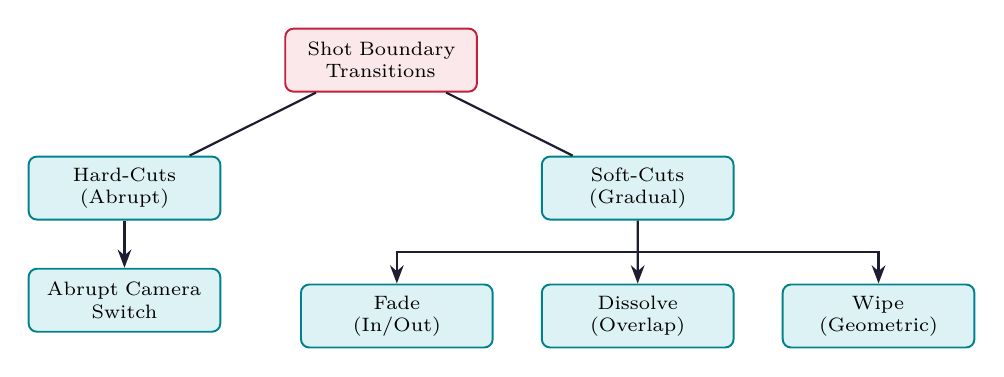
\begin{tikzpicture}[node distance=0.8cm and 0.6cm,
  sblock/.style={rectangle, draw=myteal, fill=hdrteal, text width=2.2cm,
    align=center, minimum height=0.8cm, font=\scriptsize,
    rounded corners=3pt, line width=0.7pt}]
    
  \node[sblock, draw=myred, fill=hdrred] (root) {Shot Boundary\\Transitions};
  
  \node[sblock, below left=0.8cm and 0.8cm of root] (hard) {Hard-Cuts\\(Abrupt)};
  \node[sblock, below right=0.8cm and 0.8cm of root] (soft) {Soft-Cuts\\(Gradual)};
  
  \draw[line] (root) -- (hard);
  \draw[line] (root) -- (soft);
  
  \node[sblock, below=0.6cm of hard] (cut) {Abrupt Camera\\Switch};
  \draw[arrow] (hard) -- (cut);
  
  \node[sblock, below=0.8cm of soft] (dissolve) {Dissolve\\(Overlap)};
  \node[sblock, left=0.6cm of dissolve] (fade) {Fade\\(In/Out)};
  \node[sblock, right=0.6cm of dissolve] (wipe) {Wipe\\(Geometric)};
  
  \draw[line] (soft.south) -- ($(soft.south)!0.5!(dissolve.north)$) coordinate (branch);
  \draw[arrow] (branch) -- (dissolve.north);
  \draw[arrow] (branch) -| (fade.north);
  \draw[arrow] (branch) -| (wipe.north);
\end{tikzpicture}
\end{tcolorbox}

\subsection{Detection Algorithms}
\begin{enumerate}[leftmargin=*, itemsep=3.5pt]
  \item \textbf{Pixel-Level Differencing:} Measures the average intensity change between pixels:
    \begin{equation}
      D(t, t-1) = \frac{1}{MN} \sum_{x=0}^{M-1} \sum_{y=0}^{N-1} \left| f_t(x,y) - f_{t-1}(x,y) \right|
    \end{equation}
    Highly sensitive to object and camera motion.
  \item \textbf{Histogram-Level Differencing:} Compares the intensity histograms of adjacent frames:
    \begin{equation}
      D_H(t, t-1) = \sum_{k=0}^{L-1} \left| h_t(k) - h_{t-1}(k) \right|
    \end{equation}
    Robust against minor object movements and camera pans.
  \item \textbf{Edge Change Ratio (ECR):} Measures the entry and exit of edge pixels between frames, highly effective at detecting soft-cuts.
\end{enumerate}

% ===============================================================================
\section{Spatial/Motion-Based Segmentation}
% ===============================================================================

Spatial segmentation separates moving foreground objects from static backgrounds.

\begin{itemize}[leftmargin=*, itemsep=3.5pt]
  \item \textbf{Background Subtraction:} Thresholds the difference between the current frame $f_t(x,y)$ and a reference background model $B(x,y)$:
    \begin{equation}
      |f_t(x,y) - B(x,y)| > T
    \end{equation}
    The background $B(x,y)$ is updated recursively (e.g., using Mixture of Gaussians).
  \item \textbf{Temporal Differencing:} Detects motion by subtracting adjacent frames:
    \begin{equation}
      |f_t(x,y) - f_{t-1}(x,y)| > T
    \end{equation}
    More adaptive to dynamic backgrounds, but fails to segment the interior of uniformly colored moving objects (the "ghosting" effect).
  \item \textbf{Optical Flow:} Computes the 2D velocity vector field representing the apparent motion of pixels. Highly complex, but provides detailed motion direction.
\end{itemize}

% ===============================================================================
\section{Video Object Detection and Tracking}
% ===============================================================================

Object tracking monitors the position and trajectory of a segmented object over time.

\begin{enumerate}[leftmargin=*, itemsep=3.5pt]
  \item \textbf{Kalman Filter:} A recursive estimator that predicts the state (position, velocity) of a moving object and corrects the prediction using noisy measurements. Operates in two steps:
    \begin{itemize}[leftmargin=1em, itemsep=1.5pt]
      \item \textit{Predict:} Project the state ahead: $\hat{\mathbf{x}}_k^- = \mathbf{A}\hat{\mathbf{x}}_{k-1}$.
      \item \textit{Correct:} Update the estimate using the measurement: $\hat{\mathbf{x}}_k = \hat{\mathbf{x}}_k^- + \mathbf{K}_k(\mathbf{z}_k - \mathbf{H}\hat{\mathbf{x}}_k^-)$.
    \end{itemize}
  \item \textbf{Mean-Shift Tracking:} A non-parametric iterative algorithm that locates the local maxima (peak) of a probability distribution (e.g., color histogram). It moves a tracking window towards the center of gravity of the target color distribution in each frame.
  \item \textbf{Particle Filters:} Uses Monte Carlo simulations (representing the target state probability distribution by a set of weighted particles) to track objects in non-Gaussian, non-linear environments.
\end{enumerate}

% ===============================================================================
\section{Worked Examples}
% ===============================================================================

\begin{tcolorbox}[examplebox, title={Temporal Differencing and Boundary Detection}]
\textbf{Problem:} Given two simplified $3 \times 3$ matrices representing consecutive video frames $F_{t-1}$ and $F_t$:
\begin{center}
  $F_{t-1} = \begin{bmatrix} 50 & 52 & 50 \\ 48 & 50 & 52 \\ 50 & 48 & 50 \end{bmatrix}, \quad
  F_t = \begin{bmatrix} 70 & 75 & 70 \\ 68 & 72 & 75 \\ 70 & 68 & 70 \end{bmatrix}$
\end{center}
\begin{enumerate}[label=(\alph*), leftmargin=*, itemsep=2.5pt]
  \item Calculate the pixel-level average difference metric $D(t, t-1)$.
  \item Given a threshold $T_{\text{cut}} = 15$, determine if a shot boundary transition is detected between these two frames.
\end{enumerate}

\par\noindent\rule{\linewidth}{0.5pt}\par
\textbf{Solution:}

\textbf{(a) Average Difference Calculation ($D(t, t-1)$):}
Subtract the matrices element-by-element and take the absolute values:
\begin{align*}
  |F_t - F_{t-1}| &= \begin{bmatrix} |70 - 50| & |75 - 52| & |70 - 50| \\ |68 - 48| & |72 - 50| & |75 - 52| \\ |70 - 50| & |68 - 48| & |70 - 50| \end{bmatrix} \\
  &= \begin{bmatrix} 20 & 23 & 20 \\ 20 & 22 & 23 \\ 20 & 20 & 20 \end{bmatrix}
\end{align*}
Now, compute the average over the 9 pixels ($MN = 9$):
\begin{equation*}
  D(t, t-1) = \frac{20 + 23 + 20 + 20 + 22 + 23 + 20 + 20 + 20}{9} = \frac{188}{9} \approx 20.89
\end{equation*}

\textbf{(b) Shot Boundary Decision:}
\begin{itemize}[leftmargin=*, itemsep=2pt]
  \item The computed average difference metric $D(t, t-1) = 20.89$.
  \item The boundary threshold $T_{\text{cut}} = 15$.
  \item Since $D(t, t-1) = 20.89 > T_{\text{cut}} = 15$, a shot boundary transition is indeed detected between frame $t-1$ and frame $t$.
\end{itemize}
\end{tcolorbox}

\newpage

% ===============================================================================
% MANDATORY QUICK REVISION PAGE
% ===============================================================================
\begin{center}
  {\large\bfseries\color{myred} Quick Revision --- Module VIII}\\[3pt]
  {\small\color{mydark} Video Segmentation $|$ PE-EC702B}
\end{center}
\noindent{\color{myred}\rule{\linewidth}{1.2pt}}
\vspace{4pt}

\begin{tcolorbox}[formulabox, title={\textbf{Key Formulas at a Glance}}]
\renewcommand{\arraystretch}{1.3}
\begin{tabularx}{\linewidth}{B{5.0cm} X}
Pixel Difference Metric & $D(t, t-1) = \frac{1}{MN} \sum_{x=0}^{M-1} \sum_{y=0}^{N-1} \left| f_t(x,y) - f_{t-1}(x,y) \right|$ \\
Histogram Difference & $D_H(t, t-1) = \sum_{k=0}^{L-1} \left| h_t(k) - h_{t-1}(k) \right|$ \\
Background Subtraction & $|f_t(x,y) - B(x,y)| > T$ \\
Temporal Differencing & $|f_t(x,y) - f_{t-1}(x,y)| > T$ \\
Kalman State Prediction & $\hat{\mathbf{x}}_k^- = \mathbf{A}\hat{\mathbf{x}}_{k-1}$ \\
Kalman Measurement Update & $\hat{\mathbf{x}}_k = \hat{\mathbf{x}}_k^- + \mathbf{K}_k(\mathbf{z}_k - \mathbf{H}\hat{\mathbf{x}}_k^-)$
\end{tabularx}
\tcbset{colbacktitle=myteal, coltitle=white}
\end{tcolorbox}

\begin{tcolorbox}[defbox, title={\textbf{One-Line Definitions}}]
\begin{itemize}[leftmargin=*, itemsep=2.5pt, topsep=0pt]
  \item \textbf{Hard-Cut:} An abrupt change between two consecutive frames due to camera switching, marking a shot boundary.
  \item \textbf{Soft-Cut:} A gradual, multi-frame transition (such as fade, dissolve, or wipe) between two video shots.
  \item \textbf{Background Subtraction:} A spatial differencing technique that isolates foreground objects by subtracting a background model.
  \item \textbf{Temporal Differencing:} Isolating motion by thresholding the difference between consecutive video frames.
  \item \textbf{Mean-Shift:} An iterative peak-search algorithm that tracks target centers by maximizing color probability distributions.
  \item \textbf{Optical Flow:} A vector field representing the apparent velocity of moving pixels across consecutive frames.
\end{itemize}
\end{tcolorbox}

\begin{tcolorbox}[exambox, title={\textbf{Frequently Asked / Viva Questions}}]
\begin{enumerate}[leftmargin=*, itemsep=3.5pt, label=\arabic*.]
  \item \Q{What is the difference between a hard-cut and a soft-cut transition?} A hard-cut is an abrupt, instantaneous shot transition occurring between two adjacent frames. A soft-cut is a gradual transition (such as a fade, dissolve, or wipe) that spans multiple frames.
  \item \Q{Why is histogram-level differencing preferred over pixel-level differencing for shot boundary detection?} Pixel-level differencing is highly sensitive to camera panning, zoom, and local object motion. Histogram-level differencing is robust to these changes since the overall color distribution remains similar.
  \item \Q{Explain the ghosting effect in temporal differencing.} If a moving object has a uniform interior color, subtracting adjacent frames yields differences only at the leading and trailing edges, leaving the interior segmented as background (hollow "ghost" region).
  \item \Q{How does Background Subtraction model dynamic elements like swaying trees?} By recursively updating the background model using a mixture of Gaussians (MoG) that models multiple intensity distributions for each pixel location.
  \item \Q{State the two phases of the Kalman Filter.} (1) The Prediction phase (projects the current state and error covariance estimate forward in time), and (2) the Correction/Measurement update phase (adjusts the estimate using the new sensor measurement).
  \item \Q{What is the role of the Kalman Gain $K_k$?} The Kalman gain decides the weighting between the predicted state estimate and the new measurement. If measurement noise is low, $K_k$ weights the measurement heavily; if high, it weights the prediction.
  \item \Q{Explain the difference between object detection and object tracking.} Object detection identifies and locates objects of interest in individual frames. Object tracking links these detections across consecutive frames to trace the object's path.
  \item \Q{How does the Mean-Shift algorithm track a target?} It iteratively computes the mean shift vector (displacement between the current window center and the color distribution's center of gravity) and shifts the window until convergence.
  \item \Q{What are the types of gradual transitions (soft-cuts) in video?} (1) Fade-in/out (gradual change from/to a solid black frame), (2) Dissolve (one scene overlaps and replaces another gradually), and (3) Wipe (a geometric line sweeps across the screen).
  \item \Q{What is the limitation of optical flow estimation?} Optical flow is computationally extremely intensive, making it difficult to implement in real-time without specialized hardware, and it is sensitive to illumination changes.
\end{enumerate}
\tcbset{colbacktitle=myteal, coltitle=white}
\end{tcolorbox}

\begin{tcolorbox}[tikzbox, title={Hard-Cut vs. Soft-Cut Shot Boundaries}]
\centering
\renewcommand{\arraystretch}{1.2}
\begin{tabularx}{\linewidth}{>{\bfseries}B{3.2cm} Y Y}
\rowcolor{hdrgray} Attribute & Hard-Cut Transition & Soft-Cut (Gradual) Transition \\
\midrule
Duration & Exactly 1 frame boundary & Spans multiple frames (typically 10-30) \\
\rowcolor{rowalt} Visual transition & Abrupt camera scene switch & Smooth fade, overlap (dissolve), or sweep (wipe) \\
Detection Metric & High spike in frame differences & Broad, low-amplitude peak in differences \\
\bottomrule
\end{tabularx}
\tcbset{colbacktitle=myteal, coltitle=white}
\end{tcolorbox}

\end{document}
